\documentclass{standalone}
\usepackage{tikz}
\usepackage{amsmath}
\DeclareMathOperator{\Real}{Re}
\DeclareMathOperator{\Imag}{Im}
\begin{document}
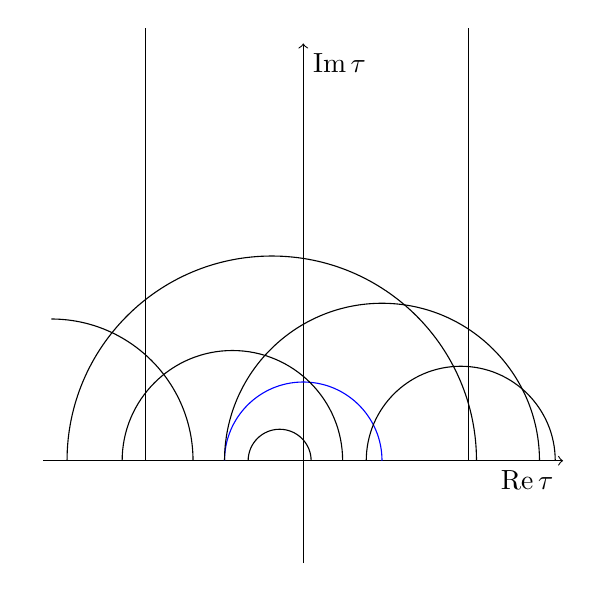
\begin{tikzpicture}
\clip (-3.5,-1.5) rectangle (3.5,5.5);

% \draw[color=gray,step=1.0,dotted] (-3.3,-3.3) grid (3.3,3.3);
\draw[->] (-3.3,0)--(3.3,0) node[below left,color=black]{$\Real \tau$};
\draw[->] (0,-1.3)--(0,5.3) node[below right]{$\Imag \tau$};

\draw[color=blue] (-1,0) arc (180:0:1);
\draw (0.8,0) arc (180:0:1.2);
\draw (-1,0) arc (180:0:2);
\draw (-2,0)--(-2,5.5);
\draw (-3,0) arc (180:0:2.6);
\draw (-3.2,1.8) arc (90:0:1.8);
\draw (2.1,0)--(2.1,5.5);
\draw (-2.3,0) arc (180:0:1.4);
\draw (-0.7,0) arc (180:0:0.4);

% \fill (2.6,2.3) circle (0.05) node[left,color=blue]{$0$} node[right,color=black]{$z_0$};
% \fill (-2.62.4) circle (0.05) node[left, color=blue]{$\infty$} node[right,color=black]{$-\bar{z}_0$};
%
% \fill (0,2) circle (0.05) node[left]{$f(1)$};
% \fill (0,-2.4) circle (0.05) node[left]{$f(-1)$};
%
% \fill (0,0) circle (0.05) node[above=5pt, right, color=blue]{$\mu$} node[below=8.5pt, left,color=black]{$0$};
% \fill (1,0) circle (0.05) node[above, color=blue]{$\alpha$} node[below=1.7pt,color=black]{$1$};
% \fill (2.1,0) circle (0.05) node[above, color=blue]{$\beta$} node[below,color=black]{$k^{-1}$};
% \fill (-1,0) circle (0.05) node[above, color=blue]{$\bar{\alpha}^{-1}$} node[below=1.7pt,color=black]{$-1$};
% \fill (-2.1,0) circle (0.05) node[above, color=blue]{$\bar{\beta}^{-1}$} node[below,color=black]{$-k^{-1}$};

\end{tikzpicture}
\end{document}
